\documentclass[
	% -- opções da classe memoir --
	12pt,				% tamanho da fonte
	oneside,			% para impressão apenas no verso. Oposto a twoside
	a4paper,			% tamanho do papel. 
	% -- opções da classe abntex2 --
	chapter=TITLE,		% títulos de capítulos convertidos em letras maiúsculas
	%section=TITLE,		% títulos de seções convertidos em letras maiúsculas
	%subsection=TITLE,	% títulos de subseções convertidos em letras maiúsculas
	%subsubsection=TITLE % títulos de subsubseções convertidos em letras maiúsculas
	% -- opções do pacote babel --
	english,			% idioma adicional para hifenização
	brazil,				% o último idioma é o principal do documento
	sumario=tradicional
	]{abntex2}


% ------------------------------------
% PACOTES
% ------------------------------------

% Pacotes fundamentais 
\usepackage{lmodern}			% Usa a fonte Latin Modern
\usepackage[T1]{fontenc}		% Selecao de codigos de fonte.
\usepackage{tikz}
\usepackage[utf8]{inputenc}		% Codificacao do documento (conversão automática dos acentos)
\usepackage{indentfirst}		% Indenta o primeiro parágrafo de cada seção.
\usepackage{color}				% Controle das cores
\usepackage{graphicx}			% Inclusão de gráficos
\usepackage{microtype} 			% para melhorias de justificação
\usepackage{folha-estilo} 	    % fomato específico relatório 
% Pacotes adicionais, usados no anexo do modelo de folha de identificação
\usepackage{multicol}
\usepackage{multirow}
\usepackage{subcaption}
\usetikzlibrary{shapes.geometric, arrows.meta, positioning, fit, backgrounds}
	
% Pacotes adicionais, usados apenas no âmbito do Modelo Canônico do abnteX2
\usepackage{lipsum}				% para geração de dummy text

% ==========================================================
% FONTE: Times New Roman (texto e matemática)
% ==========================================================
% Opção recomendada para ficar "estilo Times" em LaTeX:
\usepackage{newtxtext}
\usepackage{newtxmath}
\usepackage{enumerate} % para enumerar com letrar e etc.

% ==========================================================
% MARGENS ABNT (NBR 14724)
% Esquerda/Superior: 3 cm | Direita/Inferior: 2 cm
% ==========================================================
\usepackage[
	left=3cm,
	top=3cm,
	right=2cm,
	bottom=2cm
]{geometry}

% ── Estilos ──────────────────────────────────────────────────────────────────
\tikzset{
  % Bloco principal
  bloco/.style={
    rectangle, rounded corners=6pt,
    minimum width=3.6cm, minimum height=1.1cm,
    text centered, font=\small\bfseries,
    line width=0.5pt
  },
  % Subtítulo dentro do bloco (nó auxiliar)
  sub/.style={font=\scriptsize},
  % Seta padrão
  seta/.style={
    -{Latex[length=2mm, width=1.5mm]},
    line width=0.8pt
  },
  % Seta tracejada (efeito colateral)
  setad/.style={
    -{Latex[length=2mm, width=1.5mm]},
    line width=0.6pt, dashed, opacity=0.6
  },
  % Cores dos blocos
  coral/.style={fill=orange!15, draw=orange!60!red},
  amber/.style={fill=yellow!20, draw=orange!70},
  teal/.style={fill=teal!15,   draw=teal!60},
  blue/.style={fill=blue!10,   draw=blue!50},
  gray/.style={fill=gray!10,   draw=gray!50},
  % Contorno dos domínios
  dominio/.style={
    rectangle, rounded corners=10pt,
    draw, dashed, line width=0.7pt,
    inner sep=10pt
  }
}

% ==========================================================
% ESPAÇAMENTO ENTRE LINHAS
% (muito comum: 1,5 no texto)
% ==========================================================
\usepackage{setspace}

% ==========================================================
% RECUO DE PARÁGRAFO E ESPAÇO ENTRE PARÁGRAFOS
% ==========================================================
\setlength{\parindent}{1.25cm}
\setlength{\parskip}{0pt}

% ==========================================================
% SUMÁRIO E LINKS (PDF)
% ==========================================================
\usepackage{hyperref}
\definecolor{black}{RGB}{0,0,0}
\makeatletter
\hypersetup{
     	%pagebackref=true,
		pdftitle={\@title}, 
		pdfauthor={\@author},
    	pdfsubject={\imprimirpreambulo},
	    pdfcreator={LaTeX with abnTeX2},
		pdfkeywords={abnt}{latex}{abntex}{abntex2}{relatório técnico}, 
		colorlinks=true,       		% false: boxed links; true: colored links
    	linkcolor=black,          	% color of internal links
    	citecolor=black,        		% color of links to bibliography
    	filecolor=black,      		% color of file links
		urlcolor=black,
		bookmarksdepth=4
}
\makeatother

% Espaçamentos entre linhas e parágrafos 

% O tamanho do parágrafo é dado por:
\setlength{\parindent}{1.3cm}

% Controle do espaçamento entre um parágrafo e outro:
\setlength{\parskip}{0.2cm}  % tente também \onelineskip

% ==========================================================
% CITAÇÕES ABNT
% ==========================================================
\usepackage[brazilian,hyperpageref]{backref}	 % Paginas com as citações na bibl
\usepackage[alf]{abntex2cite}	% Citações padrão ABNT

\usepackage{caption}
\usepackage{subcaption}

% ------------------------------------
% CONFIGURAÇÕES DE PACOTES
% ------------------------------------

% Configurações do pacote backref
% Usado sem a opção hyperpageref de backref
\renewcommand{\backrefpagesname}{Citado na(s) página(s):~}
% Texto padrão antes do número das páginas
\renewcommand{\backref}{}
% Define os textos da citação
\renewcommand*{\backrefalt}[4]{
	\ifcase #1 %
		Nenhuma citação no texto.%
	\or
		Citado na página #2.%
	\else
		Citado #1 vezes nas páginas #2.%
	\fi}%


% Informações de dados para CAPA
\titulo{Processamento Digital de Sinais}
\newcommand{\professor}{Luciana Ribeiro Veloso}


% ---------------------------------------------------
%Inserir nomes dos autores aqui
\autor{Marcos Eduardo Araújo \\ Mat.: 121210541}
% ---------------------------------------------------
\local{Campina Grande, Paraíba, Brasil}
\data{2026}
\tipotrabalho{Processamento Digital de Sinais}
\preambulo{
Relatório da Disciplina: \textbf{\disciplina}.\\
Professor(a): \textbf{\professor}.\\
}



% compila o indice
\makeindex

% Início do documento
\begin{document}

% Seleciona o idioma do documento (conforme pacotes do babel)
%\selectlanguage{english}
\selectlanguage{brazil}

% Retira espaço extra obsoleto entre as frases.
\frenchspacing 



% ----------------------------------------------------------
% ELEMENTOS PRÉ-TEXTUAIS
% ----------------------------------------------------------

% Capa
\imprimircapa

% inserir o sumario
\pdfbookmark[0]{\contentsname}{toc}
\tableofcontents*
\cleardoublepage



% ----------------------------------------------------------
% ELEMENTOS TEXTUAIS
% ----------------------------------------------------------
\textual

\chapter{Introdução}
\label{sec:introducao}

O rádio definido por software (\textit{Software-Defined Radio}, SDR) é uma arquitetura de sistema de rádio em que funções tradicionalmente resolvidas por hardware dedicado — sintonia, filtragem e demodulação — são implementadas em software. O sinal é digitalizado o mais cedo possível na cadeia de recepção, por um conversor analógico-digital, o que torna o sistema reconfigurável: mudar o canal sintonizado, a largura de banda ou o esquema de demodulação passa a ser uma questão de trocar coeficientes e rotinas, e não de substituir circuitos.

Como consequência dessa escolha de arquitetura, uma fatia relativamente larga do espectro é digitalizada de uma só vez, e a separação entre os diversos canais presentes nessa faixa deixa de ser um problema de circuitos e passa a ser um problema puramente algorítmico — resolvido por filtros digitais.

\section{Motivação}

Considera-se um receptor que digitaliza uma banda de $F_s = 1{,}92$~MHz contendo múltiplos canais adjacentes. Nessa janela há vários canais transmitindo lado a lado, como estações de rádio vizinhas. Após a conversão descendente digital (\textit{Digital Down-Conversion}, DDC), o canal de interesse é trazido para a banda base, resultando em um sinal complexo em fase e quadratura (I/Q) centrado em $0$~Hz e ocupando aproximadamente $\pm 100$~kHz. O DDC, porém, apenas escolhe um dos canais: os vizinhos continuam presentes no sinal digitalizado. Um canal adjacente permanece centrado em $200$~kHz e um interferente de amplitude elevada permanece centrado em $450$~kHz, ambos dentro da faixa digitalizada.

Como o conteúdo útil do sinal ocupa uma banda muito menor do que a taxa de amostragem original, o sinal encontra-se significativamente sobreamostrado. Isso representa um custo computacional desnecessário para o bloco subsequente da cadeia de recepção — tipicamente um classificador automático de modulação, que opera sobre a constelação I/Q do sinal recebido. Propõe-se, portanto, reduzir a taxa de amostragem por meio de uma decimação de fator $M = 4$, levando a taxa efetiva de $1{,}92$~MHz para $480$~kHz.

Antes dessa redução, entretanto, um único filtro digital passa-baixas precisa cumprir duas funções simultâneas: (i) a \textbf{seleção de canal}, isolando o sinal útil (de $0$ a $100$~kHz) e rejeitando o canal adjacente a partir de $200$~kHz; e (ii) o \textbf{anti-\textit{aliasing}} para a decimação, eliminando toda energia que, ao reduzir a taxa, dobraria sobre o canal útil — em particular, o interferente em $450$~kHz. Trata-se de um filtro passa-baixas no sentido clássico: deixa passar as frequências baixas correspondentes ao canal em banda base e atenua as altas, correspondentes aos canais vizinhos e ao interferente.

\section{Justificativa do fator de decimação}

A escolha de $M = 4$ não é arbitrária: decorre de um compromisso entre o limite imposto pelo teorema da amostragem, o custo computacional do filtro e a margem operacional exigida pelo bloco seguinte. Como o sinal em banda base é complexo, a taxa mínima que preserva a informação corresponde à própria largura de banda ocupada, e não ao seu dobro; um fator $M = 8$ ($F_s' = 240$~kHz) ainda seria teoricamente admissível, pois o canal caberia dentro da nova Nyquist de $\pm 120$~kHz — deixando, porém, apenas $20$~kHz de banda de guarda de cada lado.

O custo aparece na condição de anti-\textit{aliasing}: para proteger o canal de $\pm 100$~kHz, o filtro precisa atenuar toda energia nas faixas $k\!\cdot\!(F_s/M) \pm 100$~kHz, para $k$ inteiro. Com $M = 4$, a primeira delas ($380$ a $580$~kHz) já está inteiramente coberta pela banda de rejeição exigida para bloquear o canal adjacente, e o anti-\textit{aliasing} é obtido sem exigência adicional sobre o filtro. Com $M = 8$, ela desce para o intervalo de $140$ a $340$~kHz, obrigando a banda de rejeição a começar em $140$~kHz e estreitando a faixa de transição de $100$ para $40$~kHz — o que, sendo a ordem de um FIR aproximadamente inversa a essa largura, elevaria o comprimento do filtro dos $93$ coeficientes do projeto para algo próximo de $230$. A economia na taxa de saída seria paga na filtragem.

Soma-se a isso a margem operacional: o classificador de modulação opera sobre a constelação I/Q e requer sobreamostragem em relação à taxa de símbolo — para recuperação de sincronismo, filtro casado e interpolação do instante ótimo de decisão —, e desvios residuais de frequência do estágio de DDC, bem como efeito Doppler, deslocam ligeiramente a posição espectral do canal. Os $20$~kHz de guarda de $M = 8$ seriam frágeis frente a esses desvios, enquanto $M = 4$ entrega um fator de sobreamostragem de $2{,}4$ vezes sobre a banda ocupada. O fator de decimação é, portanto, uma decisão de sistema, e não um número arbitrário do enunciado.
\section{Decimação, aliasing e folding: o perigo dos 450 kHz}
\label{sec:aliasing}

\subsection{O que a decimação faz com o espectro}

Decimar por um fator $M = 4$ significa manter uma a cada quatro amostras do sinal. Pelo teorema da amostragem, a nova taxa $F_s' = F_s/4 = 480$~kHz só representa sem ambiguidade frequências até a nova frequência de Nyquist:

\begin{equation}
f_{\mathrm{Nyq}}' = \frac{F_s'}{2} = 240 \text{ kHz}.
\end{equation}

No domínio da frequência, a decimação faz o espectro se repetir a cada $F_s' = 480$~kHz. Qualquer componente situada acima de $240$~kHz não desaparece com a operação — ela dobra (\textit{folding}) para dentro da faixa representável, sobrepondo-se ao sinal legítimo. As imagens de uma componente originalmente em uma frequência $f$ aparecem em

\begin{equation}
f_{\mathrm{alias}} = f - k \cdot F_s', \qquad k \in \mathbb{Z},
\label{eq:folding}
\end{equation}

para o valor inteiro de $k$ que traz $f_{\mathrm{alias}}$ para dentro do novo intervalo de Nyquist.

\subsection{A conta do interferente}

Aplicando a Equação~\eqref{eq:folding} ao interferente do cenário, em $450$~kHz, com $k = 1$:

\begin{equation}
f_{\mathrm{alias}} = 450 - 480 = -30 \text{ kHz}.
\end{equation}

Como o espectro é simétrico em módulo, o interferente reaparece em $\pm 30$~kHz — bem no meio do canal útil de $\pm 100$~kHz. O ponto crucial é que o \textit{aliasing} é \textbf{irreversível}: após a decimação, o interferente dobrado em $30$~kHz torna-se matematicamente indistinguível de um componente legítimo do sinal na mesma frequência, e nenhum processamento posterior é capaz de separá-los. Por essa razão, o filtro deve, obrigatoriamente, ser aplicado \emph{antes} do decimador.

A Figura~\ref{fig:diagrama-aliasing} ilustra o mecanismo. Antes da decimação, o interferente ocupa uma posição bem afastada do canal útil. Depois, ele reaparece dentro da faixa protegida, ao lado do sinal que se deseja receber.

\begin{figure}[htb]
\centering
\caption{Dobramento do interferente de $450$~kHz sobre o canal útil ao decimar por $4$.}
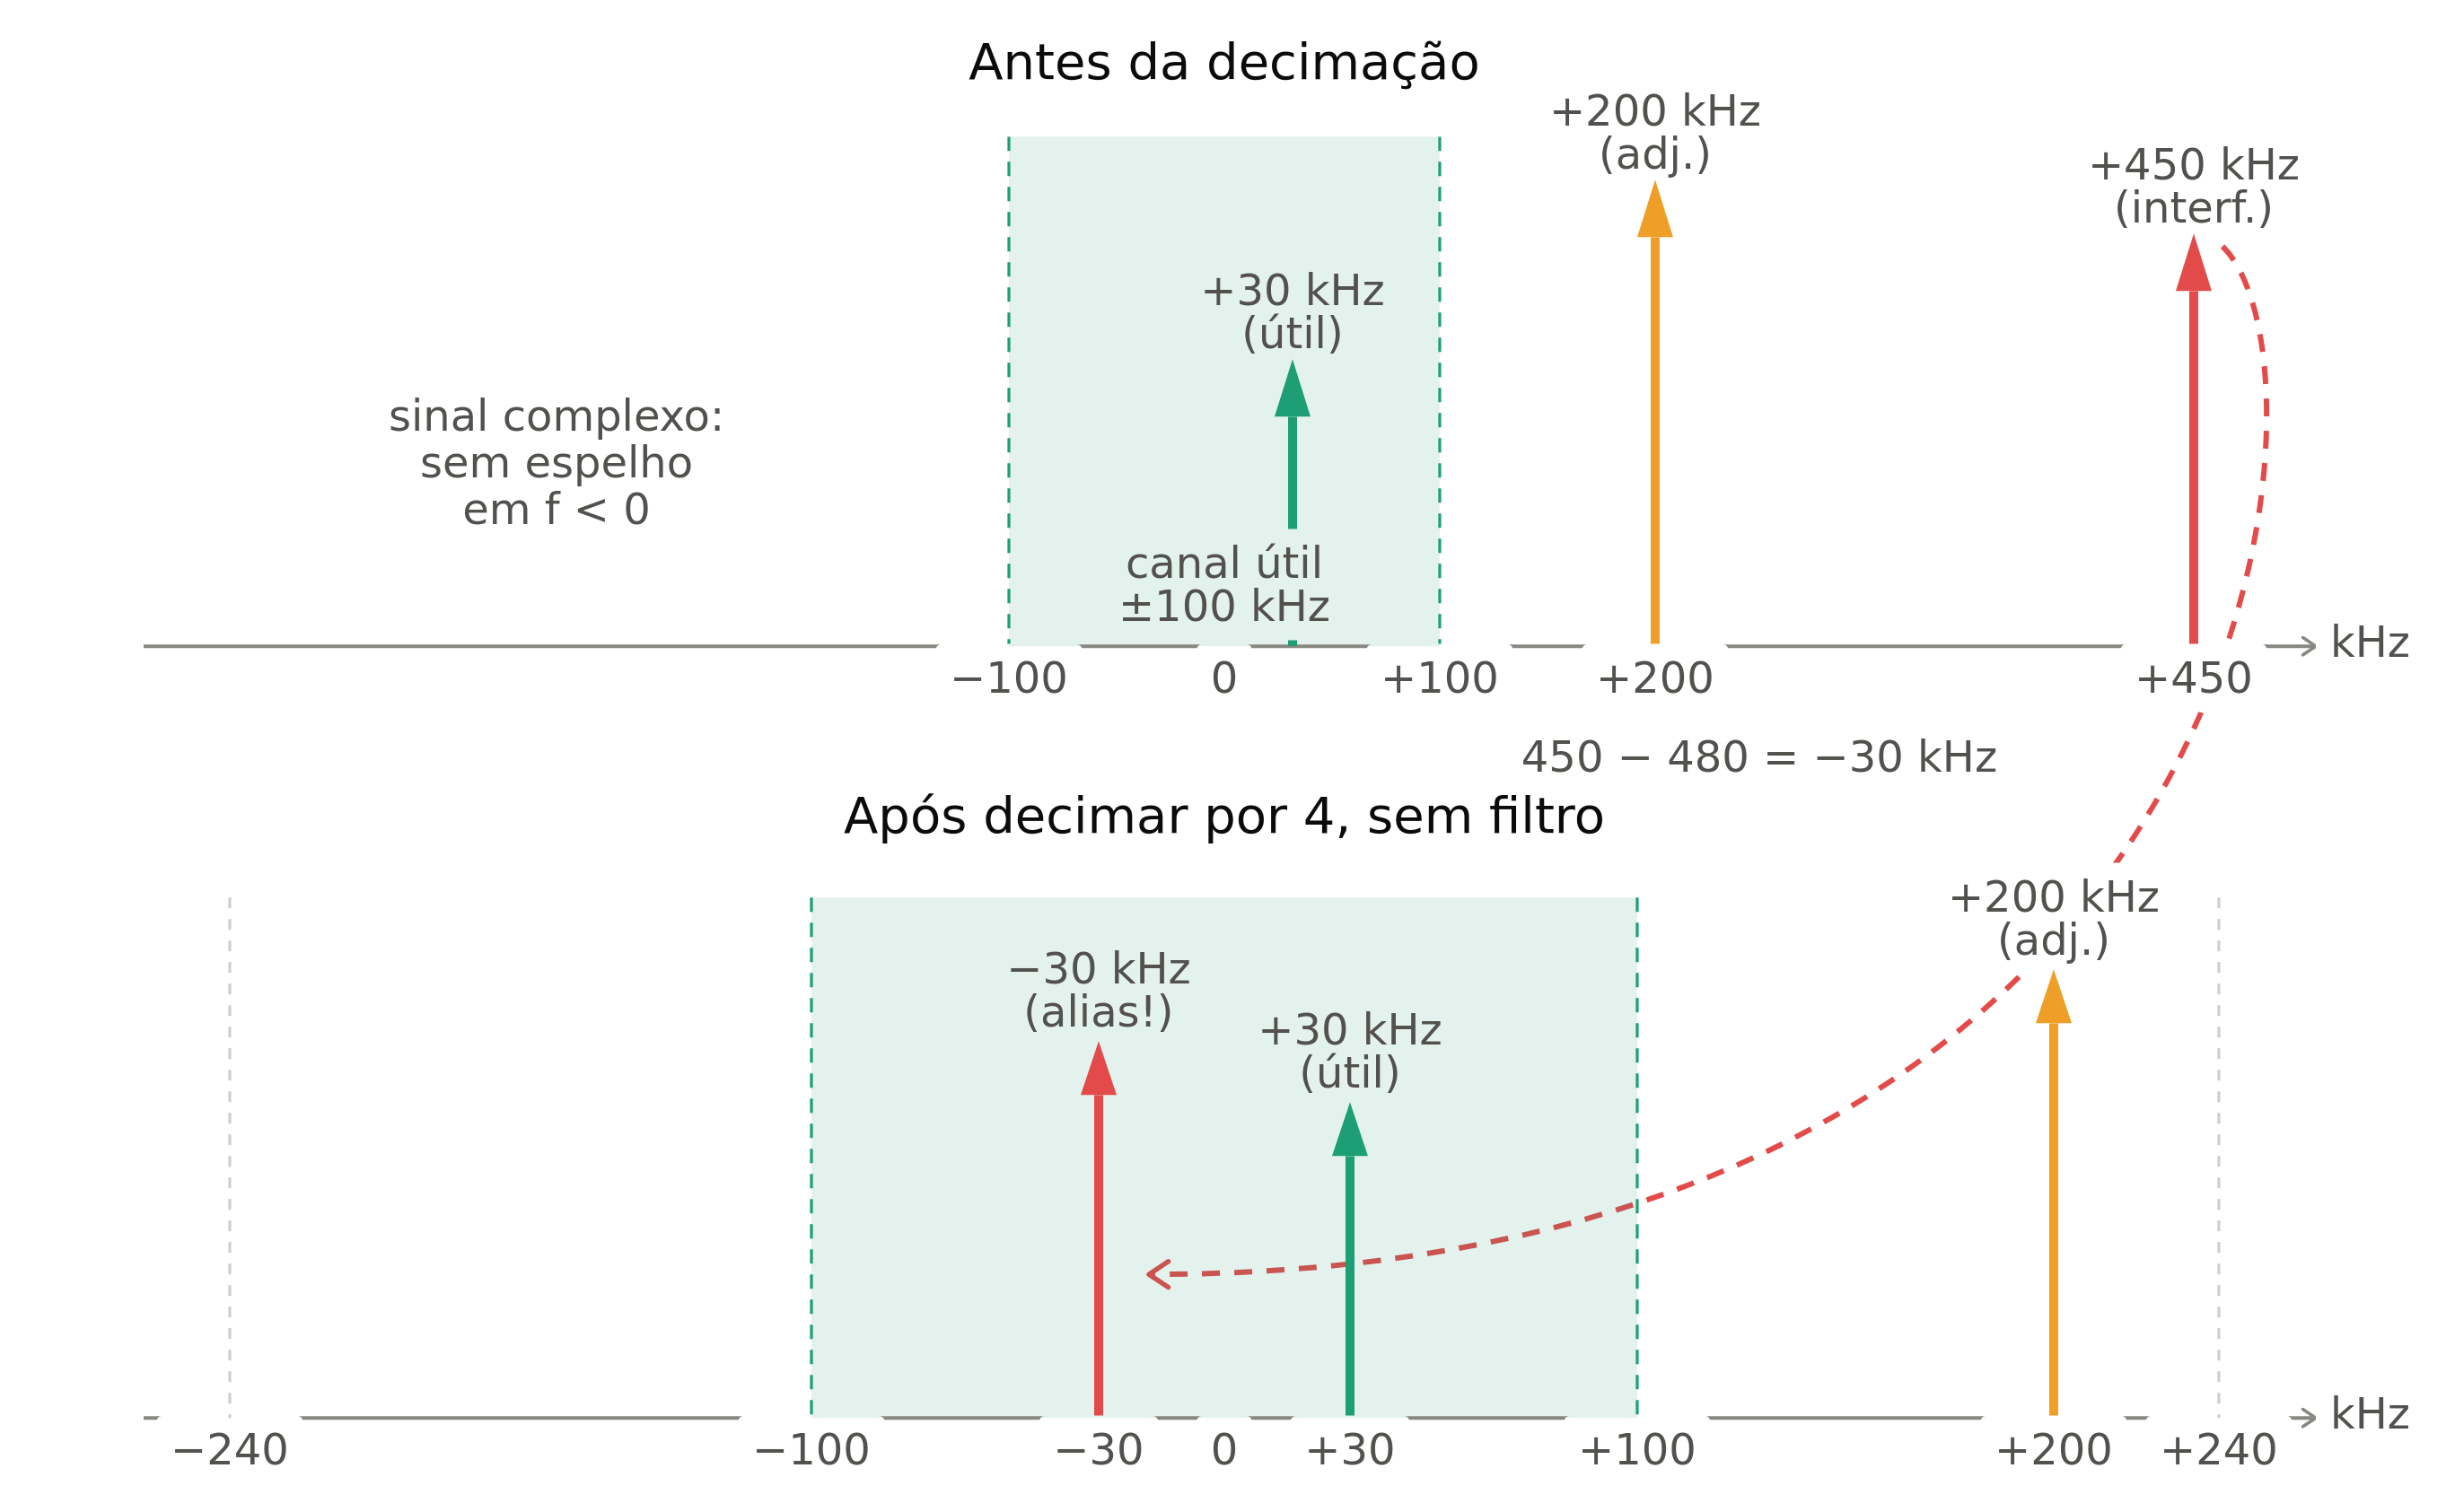
\includegraphics[width=\linewidth]{Imagens/fig00_aliasing_diagrama.png}
\label{fig:diagrama-aliasing}
\fonte{Autoria própria.}
\end{figure}

\subsection{A condição de anti-aliasing e a dupla função do filtro}

Para proteger o canal de $\pm 100$~kHz ao decimar por $4$, o filtro precisa atenuar todas as faixas espectrais que dobram sobre ele:

\begin{equation}
k \cdot 480 \pm 100 \text{ kHz}, \qquad k = 1, 2, \dots
\label{eq:faixas-proibidas}
\end{equation}

isto é, os intervalos de $380$ a $580$~kHz, de $860$ a $960$~kHz, e assim por diante.

Há aqui uma elegância de projeto digna de nota: como a banda de rejeição exigida pela seleção de canal já começa em $200$~kHz --- necessária para bloquear o canal adjacente ---, todas as faixas críticas de \textit{aliasing} dadas pela Equação~\eqref{eq:faixas-proibidas} ficam automaticamente cobertas. O filtro de seleção de canal \emph{é} o filtro de anti-\textit{aliasing}: a decimação não impõe nenhuma exigência adicional sobre a máscara de projeto.

Cabe ainda uma observação: o canal adjacente, centrado em $200$~kHz, situa-se abaixo da nova frequência de Nyquist ($240$~kHz) e, portanto, não sofre \textit{aliasing}. Sua rejeição é exigida por outro motivo — ele constitui interferência co-canal para o classificador de modulação —, e não por risco de dobramento espectral.
\section{Projeto do filtro}
\label{sec:metodologia}

\subsection{De onde saem as especificações}

O enunciado já entrega os números principais, mas vale dizer de onde cada um vem, porque nem todos estão na tabela de dados.

A faixa de passagem vai até $100$~kHz simplesmente porque é essa a banda que o canal útil ocupa ($\pm 100$~kHz em torno de zero). A faixa de rejeição começa em $200$~kHz porque é ali que está o canal vizinho, o primeiro sinal que não queremos deixar passar. Entre um e outro sobra uma faixa de transição de $100$~kHz, que é o espaço que o filtro tem para sair do ganho $1$ e chegar perto de zero.

Como o projeto é feito em tempo discreto, as frequências precisam ser normalizadas em relação à taxa de amostragem. Usando $\omega = 2\pi f / F_s$:

\begin{equation}
\omega_p = 2\pi\frac{100}{1920} = 0{,}3272 \ \mathrm{rad/amostra}, \qquad
\omega_s = 2\pi\frac{200}{1920} = 0{,}6545 \ \mathrm{rad/amostra},
\end{equation}

\begin{equation}
\Delta\omega = \omega_s - \omega_p = 0{,}3272 \ \mathrm{rad/amostra}.
\end{equation}

As tolerâncias de amplitude saem das duas exigências em decibéis. Na passagem, o ganho pode variar $0{,}1$~dB de pico a pico, o que dá

\begin{equation}
20\log_{10}\frac{1+\delta_1}{1-\delta_1} = 0{,}1 \ \mathrm{dB}
\quad \Longrightarrow \quad
\delta_1 = 0{,}0058 ,
\end{equation}

e na rejeição a atenuação de $60$~dB corresponde a

\begin{equation}
\delta_2 = 10^{-60/20} = 0{,}001 .
\end{equation}

\subsection{Uma especificação que não está na tabela}

Aqui aparece o detalhe mais importante do projeto, e ele não está escrito na lista de dados fornecidos.

O critério de aprovação pede que o interferente de $450$~kHz, depois de dobrar sobre o canal, fique $60$~dB \textbf{abaixo} do canal útil. Só que, no sinal de teste, esse interferente tem amplitude $6$ enquanto o canal útil tem amplitude $1$. Ou seja, ele já chega

\begin{equation}
20\log_{10}(6) = 15{,}56 \ \mathrm{dB}
\end{equation}

\textbf{acima} do sinal que queremos. Para ele terminar $60$~dB abaixo, o filtro não pode atenuar $60$~dB — precisa atenuar

\begin{equation}
A = 60 + 15{,}56 = 75{,}56 \ \mathrm{dB}
\label{eq:atenuacao-projeto}
\end{equation}

na região de $450$~kHz. Esse é o valor que realmente dimensiona o filtro. Projetando com os $60$~dB nominais, o filtro sai com $71$ coeficientes e o interferente termina em $-57{,}4$~dB relativos ao útil, ou seja, $2{,}6$~dB acima do limite: reprovaria no critério. Por isso a atenuação de projeto adotada foi a da Equação~\eqref{eq:atenuacao-projeto}.

Vale notar que o canal adjacente, apesar de entrar ainda mais forte ($20\log_{10}(8) = 18{,}06$~dB acima do útil), é menos exigente: ele fica fora do canal depois da decimação, então basta a rejeição de $60$~dB pedida no enunciado.

\subsection{Por que um FIR com janela de Kaiser}

O bloco seguinte da cadeia é um classificador que decide olhando a constelação I/Q, ou seja, olhando amplitude e fase dos símbolos. Se o filtro atrasar cada frequência de um jeito diferente, os pontos da constelação saem do lugar e se espalham, e o classificador erra. Um filtro FIR com coeficientes simétricos resolve isso de graça: a fase dele é uma reta e o atraso é o mesmo para todas as frequências. O sinal sai apenas deslocado no tempo, sem deformação.

Um filtro IIR teria ordem bem menor, mas a fase dele não é linear, e ainda por cima ele não se decompõe em forma polifásica (o motivo está detalhado na Seção~\ref{sec:conceitual}). Por isso a escolha foi o FIR.

Entre os métodos de janelamento, a janela de Kaiser é a única com um parâmetro ajustável. As janelas fixas entregam sempre a mesma atenuação — retangular $21$~dB, Hanning $44$~dB, Hamming $53$~dB, Blackman $74$~dB — então ou não atendem o que precisamos, ou atendem com sobra e cobram coeficientes a mais por isso. Na Kaiser, o parâmetro $\beta$ é calculado a partir da atenuação exigida, e o filtro sai com o menor comprimento possível dentro do método.

\subsection{As contas do projeto}

O procedimento seguido é o dos slides da disciplina. Com $\delta = \delta_2$ e a atenuação de projeto da Equação~\eqref{eq:atenuacao-projeto}, calcula-se primeiro o parâmetro da janela, que para $A > 50$~dB vale

\begin{equation}
\beta = 0{,}1102\,(A - 8{,}7) = 7{,}3683 ,
\end{equation}

e depois o comprimento do filtro, que depende da largura da faixa de transição:

\begin{equation}
M \simeq \frac{A - 7{,}95}{2{,}285\,\Delta\omega} + 1 = 91{,}42 \quad \Longrightarrow \quad M = 93 .
\end{equation}

O valor foi arredondado para cima e forçado a ímpar, para que o atraso

\begin{equation}
\alpha = \frac{M-1}{2} = 46 \ \mathrm{amostras}
\end{equation}

seja um número inteiro de amostras (filtro de Tipo I).

A frequência de corte do filtro ideal é colocada no meio da faixa de transição,

\begin{equation}
\omega_c = \frac{\omega_p + \omega_s}{2} = 0{,}4909 \ \mathrm{rad/amostra} \qquad (f_c = 150 \ \mathrm{kHz}),
\end{equation}

e a resposta ao impulso final é o produto do passa-baixas ideal pela janela:

\begin{equation}
h(n) = \underbrace{\frac{\mathrm{sen}\big(\omega_c(n-\alpha)\big)}{\pi(n-\alpha)}}_{\text{filtro ideal}}
\cdot
\underbrace{\frac{I_0\!\left[\beta\sqrt{1 - \left(1 - \frac{2n}{M-1}\right)^2}\right]}{I_0[\beta]}}_{\text{janela de Kaiser}},
\qquad 0 \le n \le M-1 .
\label{eq:hn}
\end{equation}

A função $I_0$ é a Bessel modificada de primeira espécie e ordem zero, calculada pela série

\begin{equation}
I_0(x) = 1 + \sum_{k=1}^{\infty}\left[\frac{(x/2)^k}{k!}\right]^2 ,
\end{equation}

que converge rápido: para $\beta = 7{,}37$ os termos já caem abaixo de $10^{-11}$ por volta do vigésimo, então uma soma com poucas dezenas de termos dá precisão de máquina.

A Figura~\ref{fig:projeto} mostra o resultado dessas contas. No canto superior esquerdo está a janela, que vale quase zero nas bordas e $1$ no centro. No canto superior direito aparece o filtro ideal (tracejado) e o filtro final (cheio): a janela vai suavizando as oscilações da ponta, e é isso que derruba os lóbulos laterais. Embaixo, à esquerda, a resposta em frequência já pronta contra a máscara de especificação, e à direita um zoom da faixa de passagem mostrando que a ondulação é muito menor que o limite.

\begin{figure}[htb]
\centering
\caption{Etapas do projeto: janela de Kaiser, resposta ao impulso e verificação contra a máscara de especificação.}
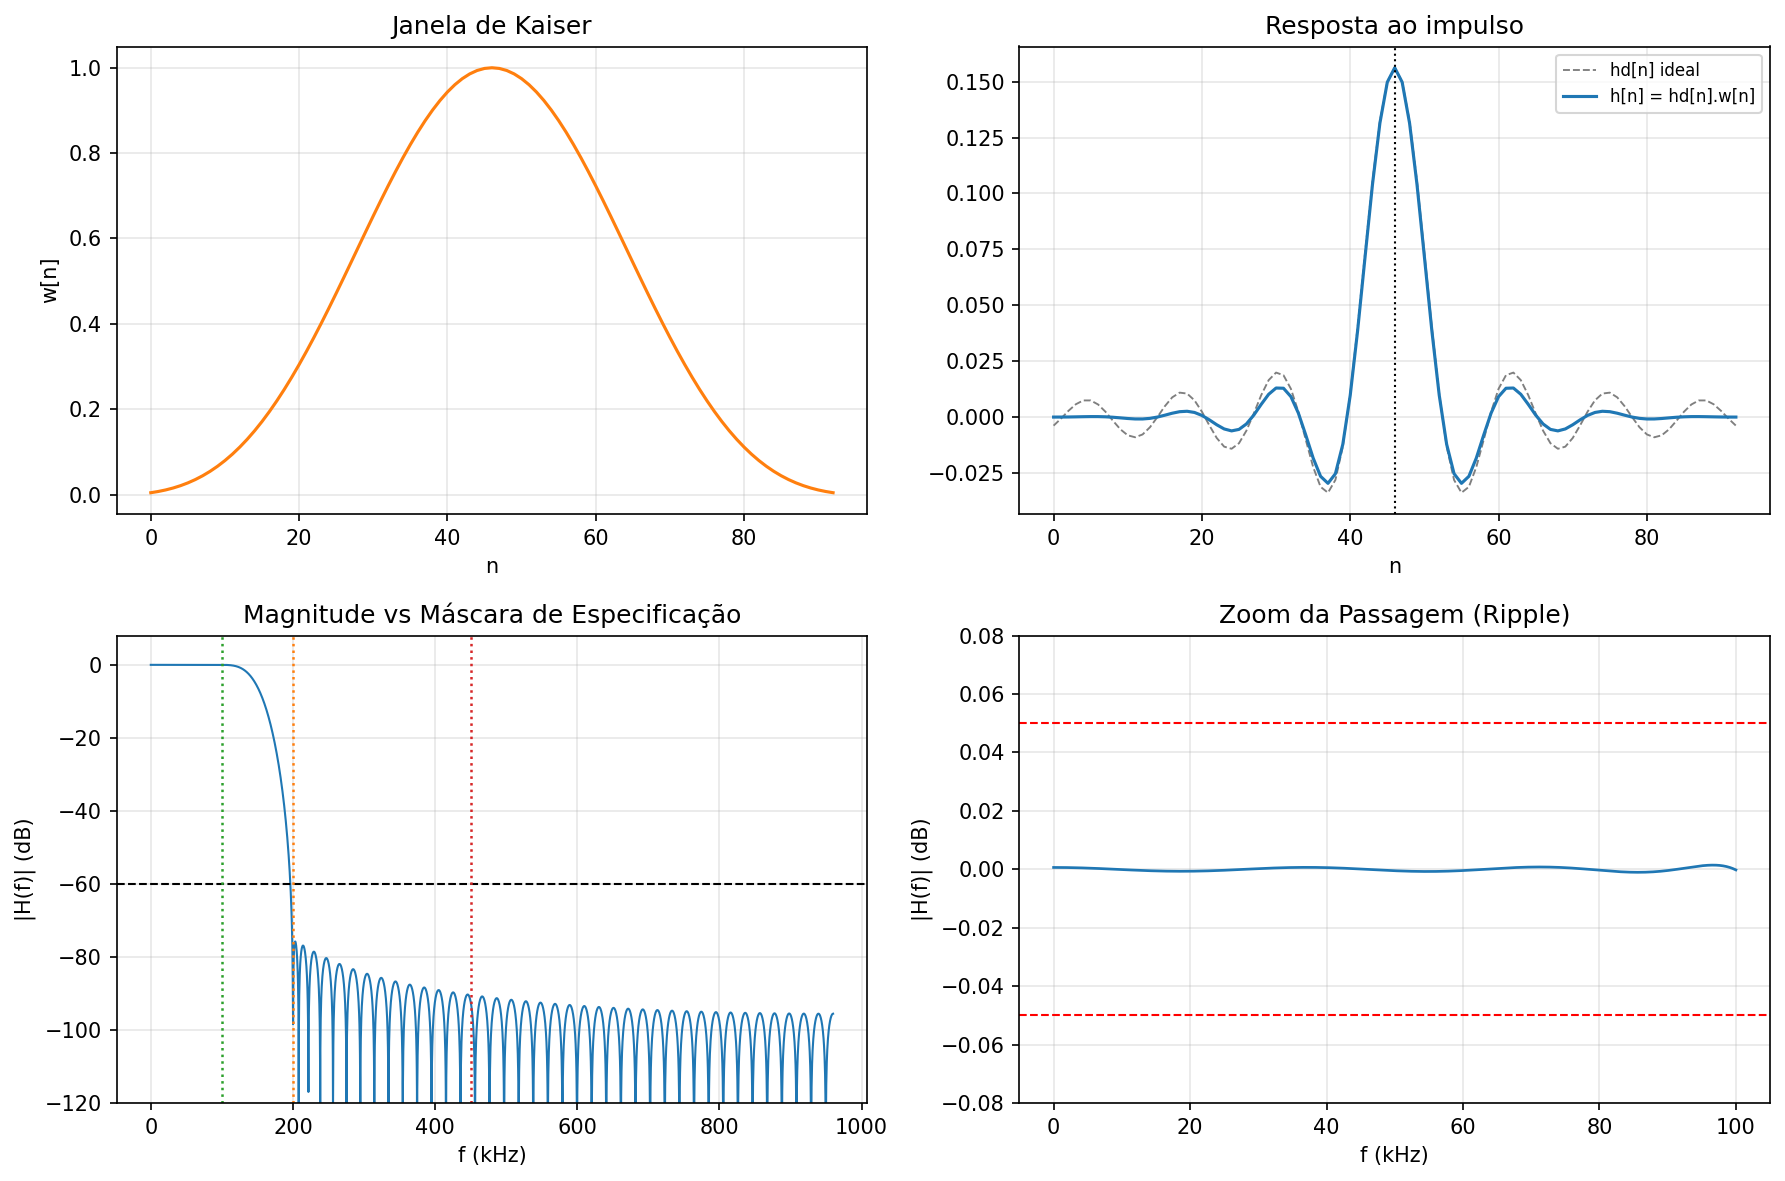
\includegraphics[width=\linewidth]{Imagens/fig02_projeto_filtro.png}
\label{fig:projeto}
\fonte{Autoria própria.}
\end{figure}

Os parâmetros obtidos estão reunidos na Tabela~\ref{tab:parametros}.

\begin{table}[htb]
\centering
\caption{Parâmetros do filtro projetado.}
\label{tab:parametros}
\begin{tabular}{ll}
\hline
\textbf{Parâmetro} & \textbf{Valor} \\
\hline
Tolerância de projeto $\delta$ & $0{,}001$ \\
Atenuação exigida pelo canal adjacente & $60{,}00$~dB \\
Atenuação exigida pelo interferente & $75{,}56$~dB \\
Atenuação de projeto $A$ & $75{,}56$~dB \\
Parâmetro da janela $\beta$ & $7{,}3683$ \\
Comprimento $M$ & $93$ coeficientes \\
Atraso $\alpha$ & $46$ amostras ($23{,}96$~$\mu$s) \\
Frequência de corte $f_c$ & $150$~kHz ($\omega_c = 0{,}4909$) \\
\hline
\end{tabular}
\fonte{Autoria própria.}
\end{table}

\section{Resultados}
\label{sec:resultados}

\subsection{O sinal de teste}

O sinal usado é o do enunciado, gerado com a semente indicada para que o resultado seja reprodutível. Ele é a soma de quatro coisas: o canal útil em $30$~kHz com amplitude $1$ e uma pequena modulação de amplitude, o canal adjacente em $200$~kHz com amplitude $8$, o interferente em $450$~kHz com amplitude $6$ e um ruído fraco de amplitude $0{,}01$.

A Figura~\ref{fig:sinal} mostra esse sinal de duas maneiras. Em cima, no tempo: as partes real (I) e imaginária (Q) somadas dão uma forma de onda embaralhada, com picos passando de $15$, e é impossível enxergar o canal útil no meio disso — ele tem amplitude $1$ contra vizinhos de amplitude $8$ e $6$. Embaixo, no espectro, cada componente aparece separada na sua frequência, e o desenho fica imediatamente legível.

\begin{figure}[htb]
\centering
\caption{Sinal recebido em banda base: no tempo (acima) e no espectro (abaixo), com $0$~dB tomado no canal útil.}
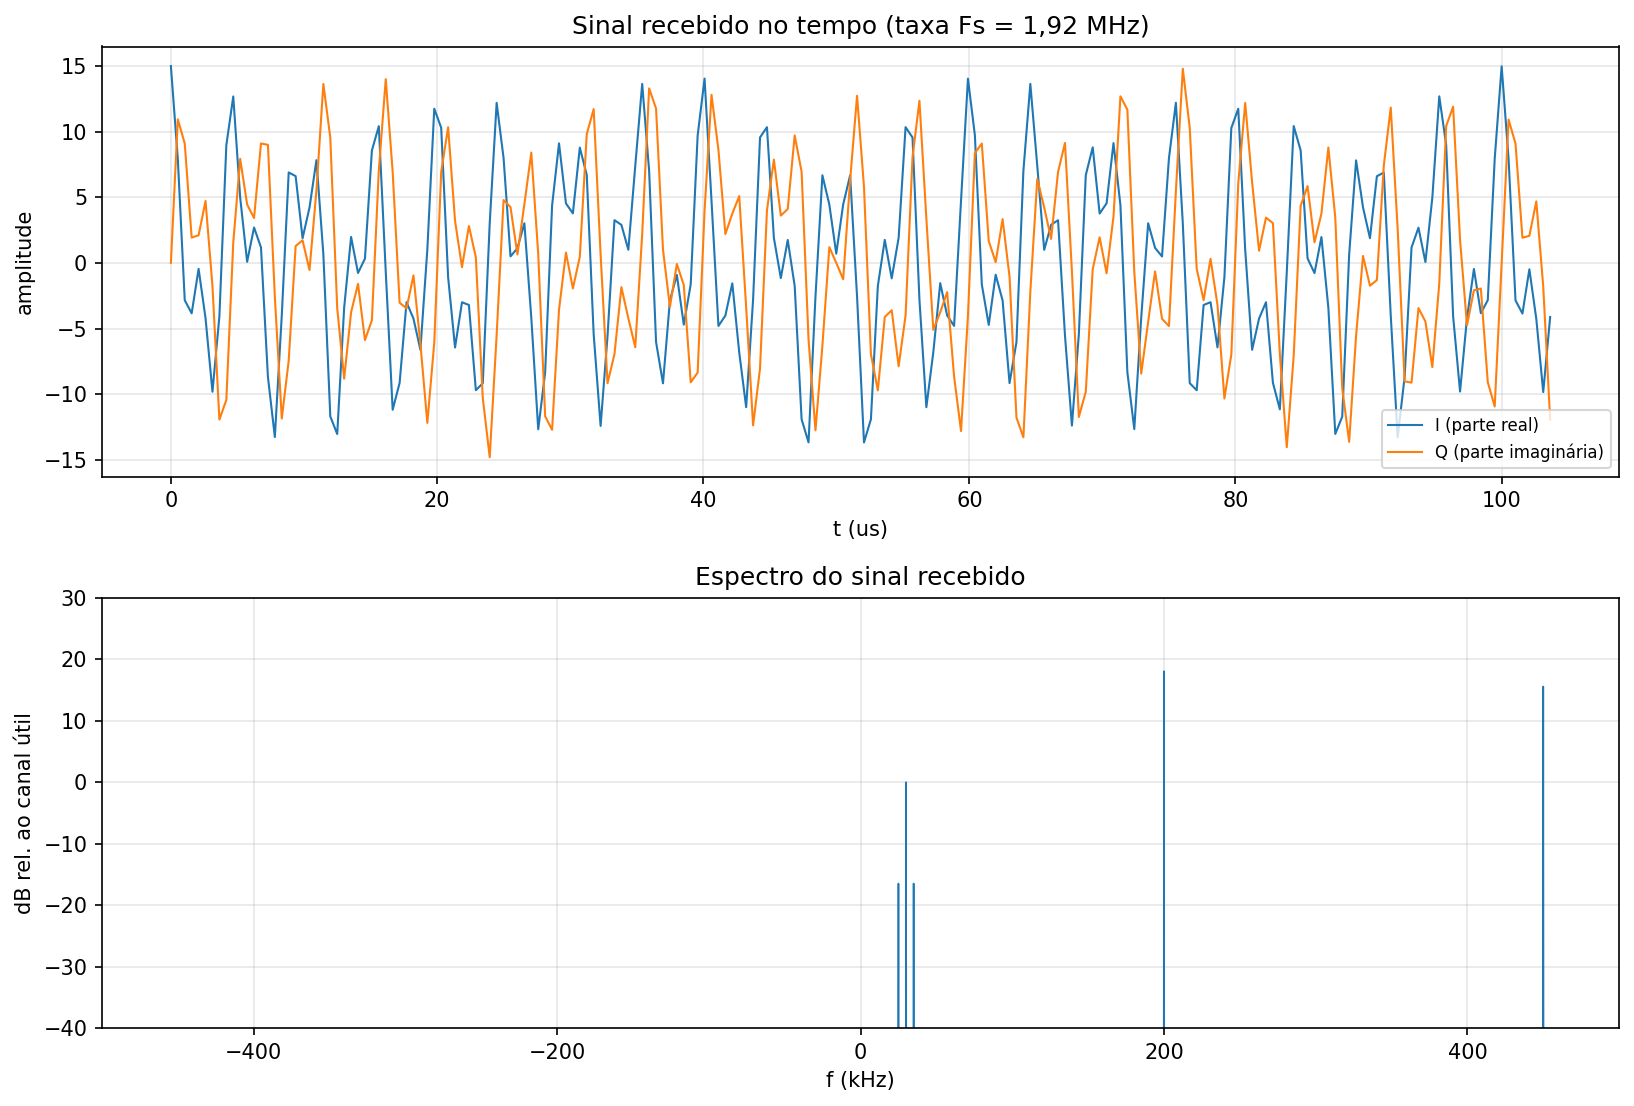
\includegraphics[width=\linewidth]{Imagens/fig01_sinal_recebido.png}
\label{fig:sinal}
\fonte{Autoria própria.}
\end{figure}

Vale explicar por que cada raia está onde está, e com aquela altura.

\begin{enumerate}[a)]
\item \textbf{A raia em $30$~kHz, no nível $0$~dB.} É o canal útil. Ela foi escolhida como referência de $0$~dB do gráfico, então todas as outras alturas são lidas em relação a ela. As duas raias menores logo ao lado, em $25$ e $35$~kHz e cerca de $16$~dB abaixo, não são um sinal separado: são as bandas laterais criadas pela modulação de amplitude. Multiplicar a portadora por $(1 + 0{,}3\,\mathrm{sen}(2\pi 5000t))$ produz duas cópias afastadas de $5$~kHz para cada lado, cada uma com amplitude $0{,}15$, o que dá exatamente $20\log_{10}(0{,}15) = -16{,}5$~dB.

\item \textbf{A raia em $200$~kHz, $18{,}1$~dB acima.} É o canal adjacente. A altura vem direto da amplitude que ele tem no sinal: $20\log_{10}(8/1) = 18{,}06$~dB. Ele está em $200$~kHz porque é a posição do canal vizinho depois que o DDC trouxe o canal de interesse para o zero.

\item \textbf{A raia em $450$~kHz, $15{,}6$~dB acima.} É o interferente forte. A altura, de novo, é só a razão de amplitudes: $20\log_{10}(6/1) = 15{,}56$~dB. A frequência não é acidental: $450$~kHz foi escolhida no enunciado justamente porque, ao decimar por $4$, ela cai exatamente em cima do canal útil.

\item \textbf{O piso em torno de $-73$~dB.} É o ruído. Ele não forma raia porque está espalhado por todas as frequências, e não concentrado em uma só.
\end{enumerate}

O ponto que esses números deixam claro é que o filtro não precisa apenas atenuar: ele precisa atenuar o suficiente para vencer a vantagem de $18$ e $15{,}6$~dB com que os interferentes chegam. Foi disso que saiu a atenuação de projeto de $75{,}56$~dB discutida na Seção~\ref{sec:metodologia}.

\subsection{A resposta em frequência do filtro}

A Figura~\ref{fig:resposta} traz os três gráficos pedidos, com as bordas de $100$ e $200$~kHz marcadas por linhas tracejadas nos três painéis.

\begin{figure}[htb]
\centering
\caption{Resposta em frequência do filtro projetado: magnitude, fase e atraso de grupo.}
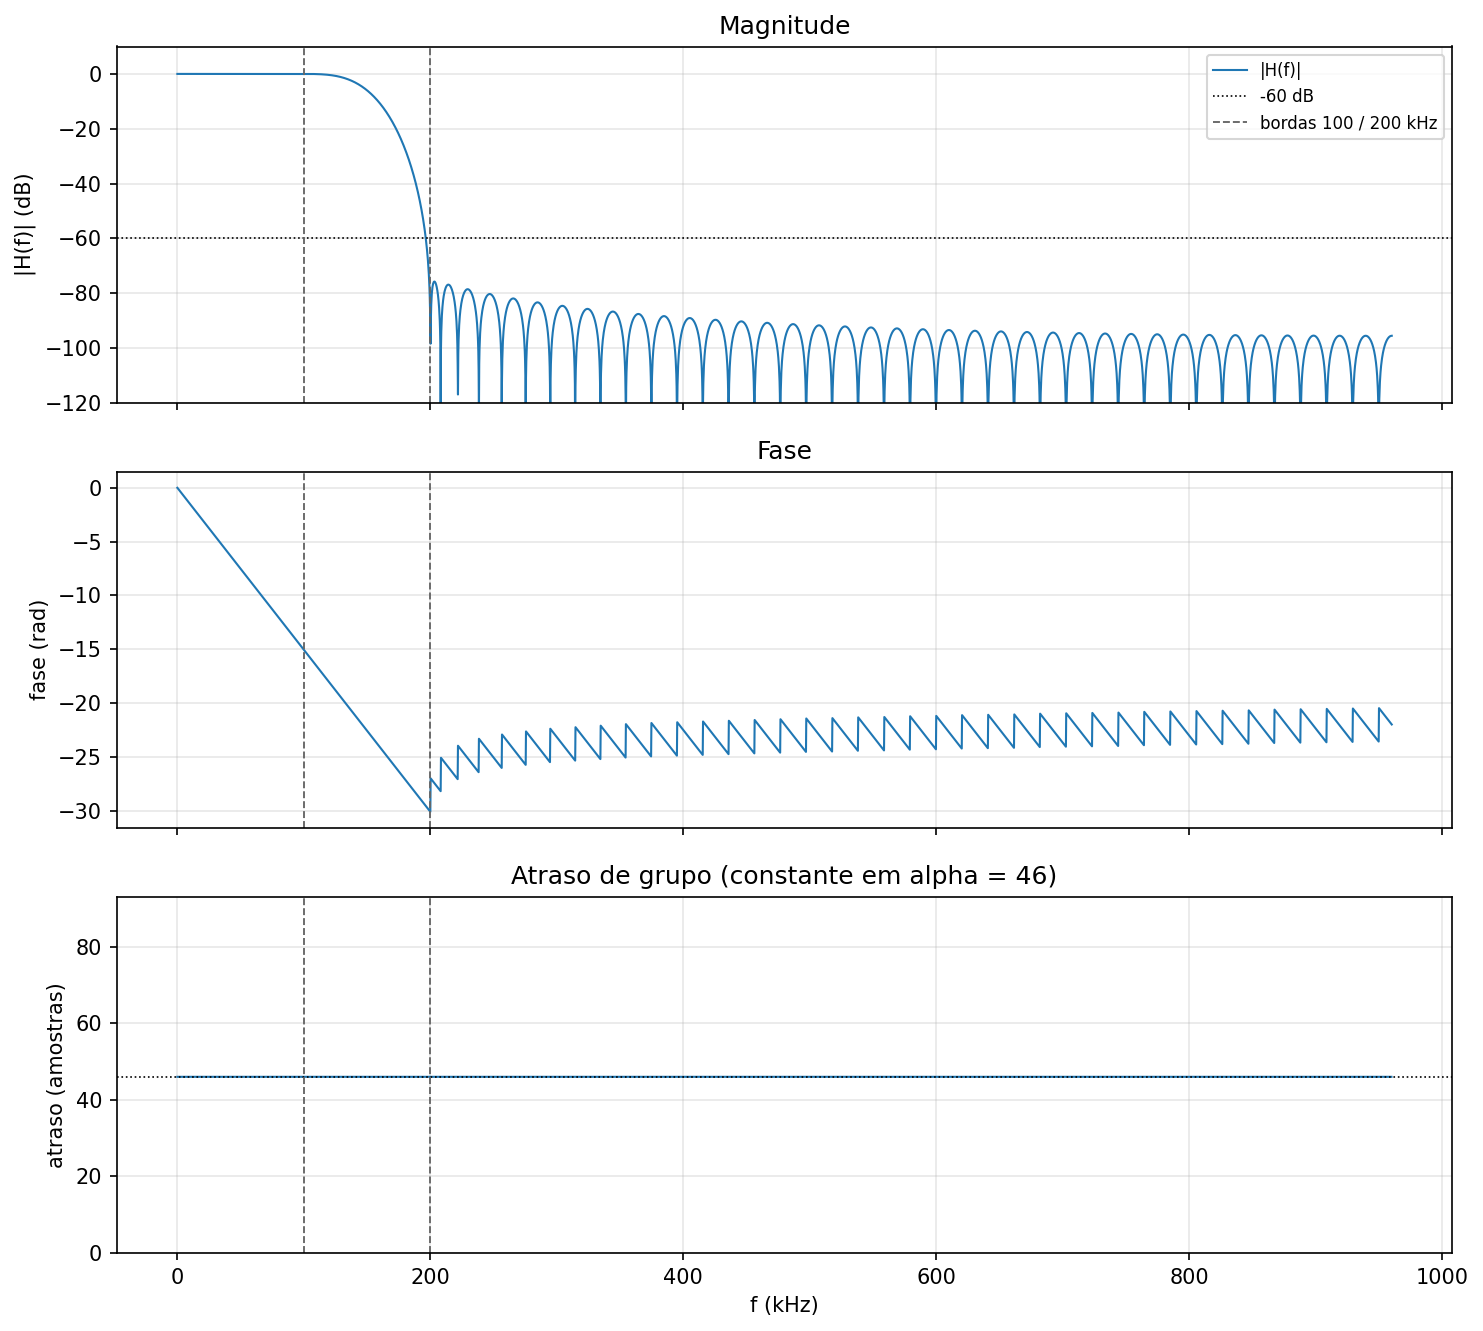
\includegraphics[width=0.92\linewidth]{Imagens/fig03_resposta_frequencia.png}
\label{fig:resposta}
\fonte{Autoria própria.}
\end{figure}

\textbf{A magnitude} (painel de cima) mostra o comportamento esperado de um passa-baixas: ganho praticamente constante até $100$~kHz, uma descida rápida na faixa de transição e, a partir de $200$~kHz, uma sucessão de lóbulos que nunca sobem acima de $-75$~dB. A linha pontilhada marca os $-60$~dB do enunciado, e dá para ver que a resposta passa bem abaixo dela — a sobra é justamente a atenuação extra que o interferente exigiu.

\textbf{A fase} (painel do meio) é uma reta descendente dentro da faixa de passagem, que é a assinatura da fase linear. Os dentes de serra que aparecem depois de $200$~kHz não são distorção: são apenas os pontos onde a magnitude passa por zero, e nesses pontos a fase salta $\pi$. Como ali o sinal já foi atenuado quase $100$~dB, não há nada de relevante acontecendo naquela região.

\textbf{O atraso de grupo} (painel de baixo) é uma reta horizontal em $46$ amostras, do início ao fim da banda. Essa é a prova visual de que o filtro não distorce a fase: todas as frequências saem atrasadas exatamente do mesmo tanto, $46$ amostras ou $23{,}96$~$\mu$s. A verificação numérica confirma: dentro da faixa de passagem, o mínimo e o máximo do atraso são ambos $46{,}0000$ amostras.

\subsection{Antes e depois do filtro}

A Figura~\ref{fig:antes-depois} mostra o efeito do filtro sobre o sinal de teste, em três recortes.

\begin{figure}[htb]
\centering
\caption{Efeito do filtro: espectro na taxa original, espectro após a decimação e comparação no tempo.}
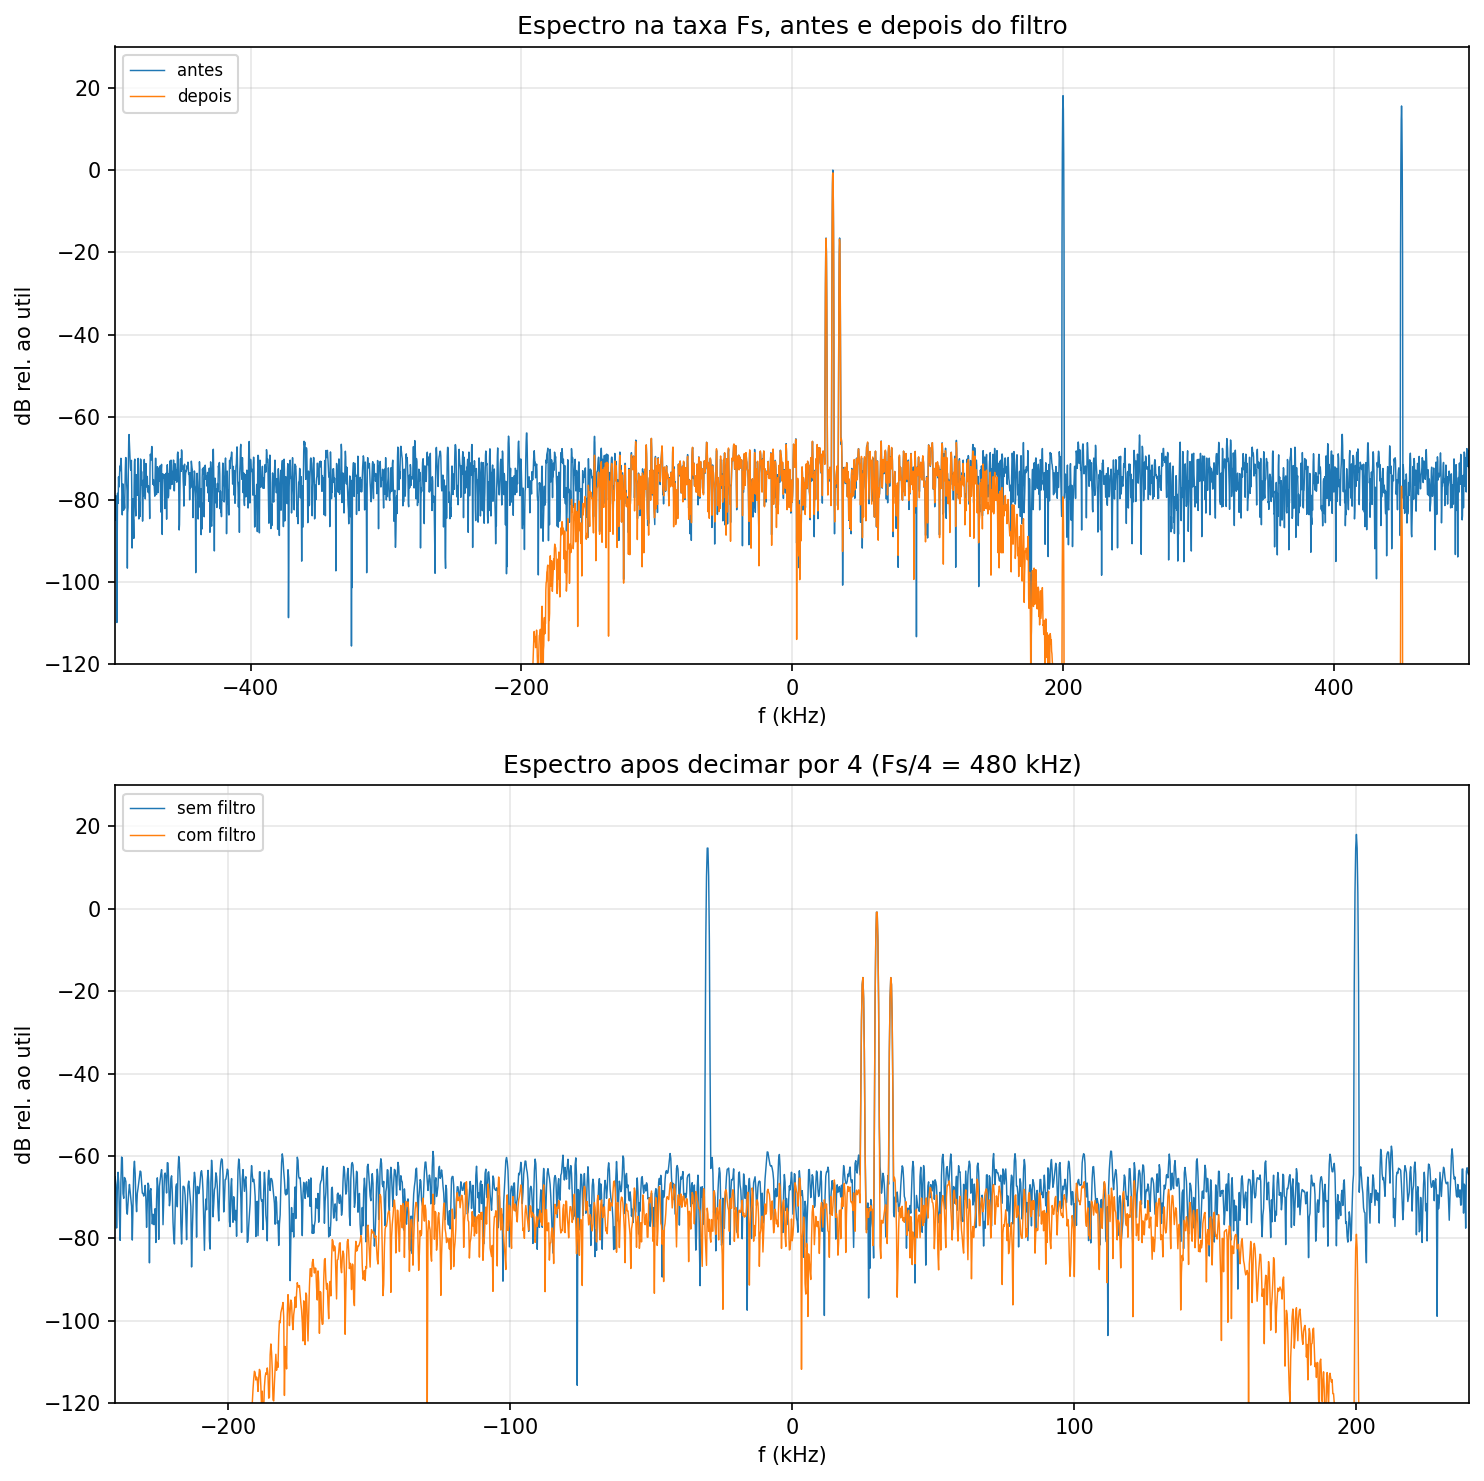
\includegraphics[width=0.92\linewidth]{Imagens/fig04_antes_depois.png}
\label{fig:antes-depois}
\fonte{Autoria própria.}
\end{figure}

No \textbf{painel de cima}, ainda na taxa de $1{,}92$~MHz, a curva ``antes'' tem as três raias descritas na Seção anterior. Na curva ``depois'', as raias de $200$ e $450$~kHz simplesmente somem, e o que resta é o canal útil com suas bandas laterais, exatamente como estavam. Repare também que o piso de ruído cai fora da banda de passagem: o filtro não elimina só os interferentes, ele elimina todo o ruído que estava fora do canal.

O \textbf{painel do meio} é o mais importante do trabalho, porque mostra o problema e a solução lado a lado. A curva ``sem filtro'' é o que aconteceria se decimássemos direto: aparece uma raia em $-30$~kHz que não existia no sinal original — é o interferente de $450$~kHz que dobrou para dentro do canal, exatamente como previsto pela conta $450 - 480 = -30$~kHz. Ela chega com $+15{,}6$~dB, ou seja, quinze decibéis mais forte que o próprio canal que queremos receber. Na curva ``com filtro'' essa raia desaparece por completo, e sobra apenas o canal útil.

O \textbf{painel de baixo} compara no tempo. A curva fina e agitada é a entrada, com os interferentes somados. A curva grossa é a saída depois de filtrar e decimar, e a tracejada é o canal útil original deslocado de $46$ amostras. As duas últimas se sobrepõem quase perfeitamente, o que mostra que o filtro tirou tudo o que sobrava sem estragar o que interessava — só atrasou. O pequeno desencontro nos primeiros microssegundos é o transiente do filtro, que precisa de $M$ amostras para encher a linha de atraso antes de entregar o resultado correto.

\subsection{Decimação polifásica}

Na implementação direta, o filtro é calculado para toda amostra que entra e depois se descarta três de cada quatro resultados. É trabalho jogado fora: cada amostra de saída custa $93 \times 4 = 372$ multiplicações, e três quartos delas produziram números que ninguém usou.

A decomposição polifásica reorganiza a mesma soma. Escrevendo a saída já decimada e separando os coeficientes segundo o resto da divisão por $4$, o filtro se quebra em quatro subfiltros de $24$ coeficientes que já trabalham na taxa baixa. Cada coeficiente passa a ser usado uma única vez por amostra de saída, e o custo cai para $96$ multiplicações — praticamente o fator $4$ da decimação (o valor exato é $3{,}9$ porque foram somados três zeros para fechar quatro ramos iguais).

O ponto importante é que não se trata de uma aproximação. Comparando a saída da implementação direta com a da polifásica, a maior diferença encontrada foi de $1{,}5 \times 10^{-15}$, que é o erro de arredondamento do ponto flutuante. As duas fazem exatamente a mesma conta.

A Figura~\ref{fig:polifasica} confirma no espectro que o resultado da polifásica está correto: dentro do canal útil, marcado pelas linhas tracejadas em $\pm 100$~kHz, não sobrou nem o interferente dobrado nem o canal adjacente.

\begin{figure}[htb]
\centering
\caption{Espectro decimado pela implementação polifásica, comparado com a decimação sem filtro.}
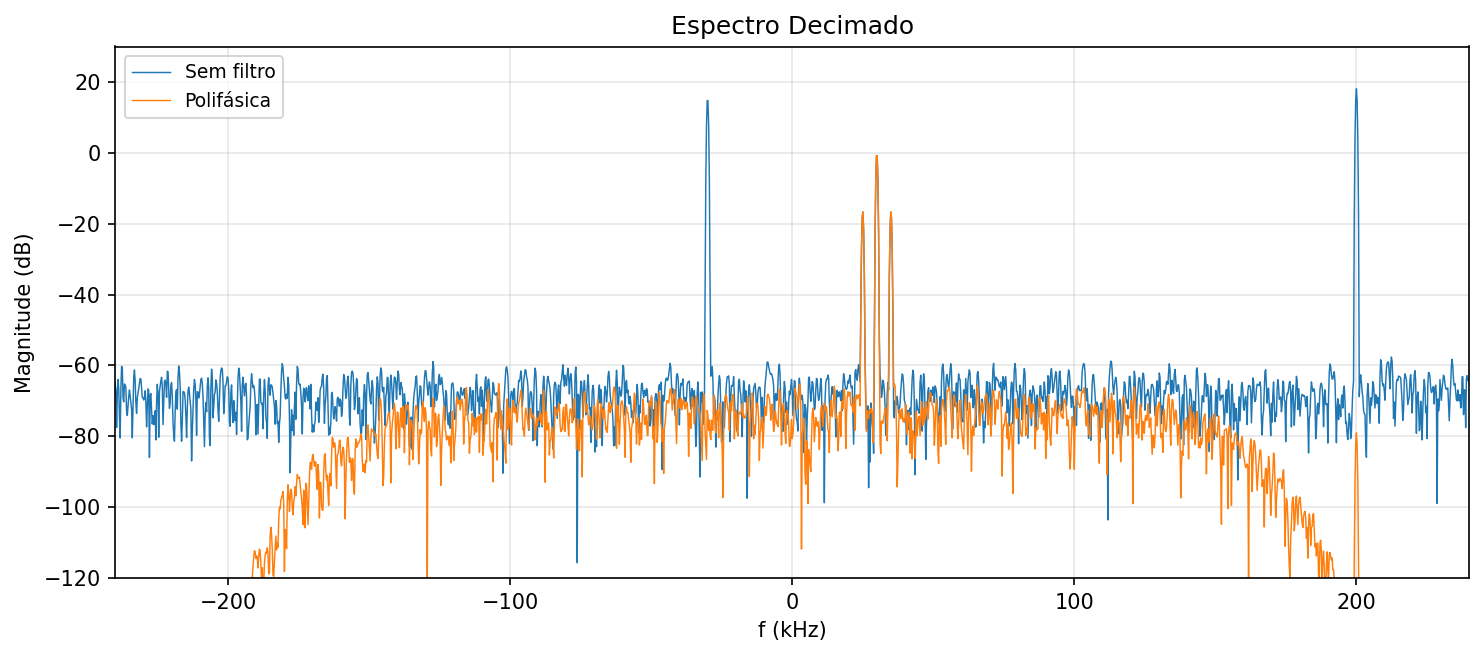
\includegraphics[width=0.92\linewidth]{Imagens/fig05_polifasica.png}
\label{fig:polifasica}
\fonte{Autoria própria.}
\end{figure}

\subsection{Tabela de métricas}

A Tabela~\ref{tab:metricas} reúne as medidas pedidas na Seção 6 do enunciado.

\begin{table}[htb]
\centering
\caption{Métricas obtidas.}
\label{tab:metricas}
\begin{tabular}{p{7.5cm}p{6cm}}
\hline
\textbf{Métrica} & \textbf{Valor obtido} \\
\hline
Número de coeficientes e atraso de grupo & $93$ coeficientes; $46$ amostras ($23{,}96$~$\mu$s) \\
Rejeição medida em $200$~kHz & $97{,}08$~dB \\
Atenuação em $450$~kHz e nível do \textit{aliasing} sobre o canal & $92{,}19$~dB; \textit{alias} em $-71{,}9$~dB abaixo do útil \\
Multiplicações por amostra de saída & $372$ (direta) contra $96$ (polifásica) \\
\hline
\end{tabular}
\fonte{Autoria própria.}
\end{table}

\subsection{Critério de aprovação}

A Tabela~\ref{tab:aprovacao} confronta os valores medidos com os três limites da Seção 7 do enunciado. Todos são atendidos.

\begin{table}[htb]
\centering
\caption{Verificação do critério de aprovação.}
\label{tab:aprovacao}
\begin{tabular}{lccc}
\hline
\textbf{Critério} & \textbf{Exigido} & \textbf{Obtido} & \\
\hline
Rejeição em $200$~kHz & $\ge 60$~dB & $97{,}08$~dB & atende \\
Componente de $450$~kHz dobrada sobre o útil & $\le -60$~dB & $-71{,}9$~dB & atende \\
Ondulação na passagem até $100$~kHz & $\pm 0{,}1$~dB & $0{,}0025$~dB & atende \\
\hline
\end{tabular}
\fonte{Autoria própria.}
\end{table}

Cabe uma observação sobre o segundo valor. A previsão teórica para o \textit{alias} é $15{,}56 - 92{,}19 = -76{,}6$~dB, mas o que se mede no gráfico é $-71{,}9$~dB. A diferença não é erro de projeto: o piso de ruído do sinal de teste está em torno de $-73$~dB, então a raia do interferente já foi empurrada para \emph{abaixo} do ruído e o que se lê naquele ponto do espectro é o próprio ruído. Em outras palavras, o interferente foi eliminado até um nível que o sinal de teste não permite mais enxergar.

\section{Questão conceitual}
\label{sec:conceitual}

\subsection{Por que a fase linear preserva a constelação I/Q}

Quando os coeficientes do filtro são simétricos, ou seja $h[n] = h[M-1-n]$, a resposta em frequência pode ser escrita como

\begin{equation}
H(e^{j\omega}) = A(\omega)\,e^{-j\omega\alpha},
\end{equation}

com $A(\omega)$ real. Toda a dependência da fase com a frequência está naquele expoente, que é uma reta. Derivando, o atraso de grupo dá

\begin{equation}
\tau(\omega) = -\frac{d\theta}{d\omega} = \alpha = 46 \ \mathrm{amostras},
\end{equation}

um valor constante, igual para todas as frequências.

Na prática isso significa que o sinal complexo inteiro sai apenas deslocado no tempo. Nenhuma componente chega antes ou depois das outras, então o símbolo que entrou íntegro sai íntegro, e os pontos da constelação continuam nas mesmas posições. O bloco seguinte só precisa saber que existe um atraso fixo de $46$ amostras, e o sincronizador dá conta disso sozinho.

Se a fase não fosse linear, cada frequência sofreria um atraso diferente. A energia de um símbolo, que deveria chegar concentrada em um instante, se espalharia pelos instantes vizinhos e invadiria os símbolos seguintes — é a interferência entre símbolos. Na constelação, os pontos apareceriam girados e borrados, cada um de um jeito. Como o classificador decide justamente pela geometria desses pontos, ele passaria a confundir uma modulação com outra, e o demodulador erraria a decisão.

\subsection{Por que a polifásica reduz o custo sem perder informação}

A economia vem de perceber que, na filtragem direta seguida de decimação, três de cada quatro resultados são calculados e jogados fora. A polifásica não descobre nenhum atalho matemático: ela apenas separa a soma de modo que só as saídas que serão usadas sejam calculadas.

Partindo da saída já decimada,

\begin{equation}
y[m] = \sum_k h[k]\,x[Dm-k],
\end{equation}

e reescrevendo o índice como $k = qD + p$, com $p$ indo de $0$ a $D-1$:

\begin{equation}
y[m] = \sum_{p=0}^{D-1}\sum_q h[qD+p]\;x[D(m-q)-p]
     = \sum_{p=0}^{D-1}\big(h_p * x_p\big)[m],
\end{equation}

onde $h_p[q] = h[qD+p]$ é o subfiltro $p$ e $x_p[m] = x[Dm-p]$ é a entrada já subamostrada. Cada um dos quatro ramos tem $M/D$ coeficientes e opera na taxa baixa. Somando os ramos, cada coeficiente de $h$ é usado uma única vez por amostra de saída, o que dá o fator $D$ de economia.

Não há perda de informação porque nenhuma parcela foi eliminada da conta: a soma é a mesma, apenas em outra ordem. É por isso que a diferença numérica entre as duas implementações fica no nível do erro de arredondamento.

\subsection{Por que um IIR seria pior aqui}

Para responder a essa parte com número, e não só com argumento, um filtro elíptico foi projetado para as \emph{mesmas} especificações do FIR e os dois foram comparados lado a lado. O elíptico atende com ordem $6$ — três seções de segunda ordem — contra os $93$ coeficientes do FIR. A diferença parece enorme, mas dois problemas anulam essa vantagem.

O primeiro é a fase, e a Figura~\ref{fig:fir-vs-iir} mostra isso de forma direta. Na magnitude (painel superior esquerdo) os dois cumprem a especificação, e o elíptico até desce mais rápido na transição — é a vantagem esperada dele. Mas na fase (painel superior direito) a diferença salta aos olhos: a do FIR é uma reta perfeita, enquanto a do IIR é curva e cheia de quebras. A consequência aparece no atraso de grupo (painéis inferiores): o FIR é uma linha horizontal em $46$ amostras, enquanto o IIR varia de $11{,}90$ a $35{,}75$ amostras dentro da faixa de passagem, ou seja, $23{,}86$ amostras de dispersão — $12{,}42$~$\mu$s.

\begin{figure}[htb]
\centering
\caption{FIR de fase linear contra IIR elíptico projetado para as mesmas especificações.}
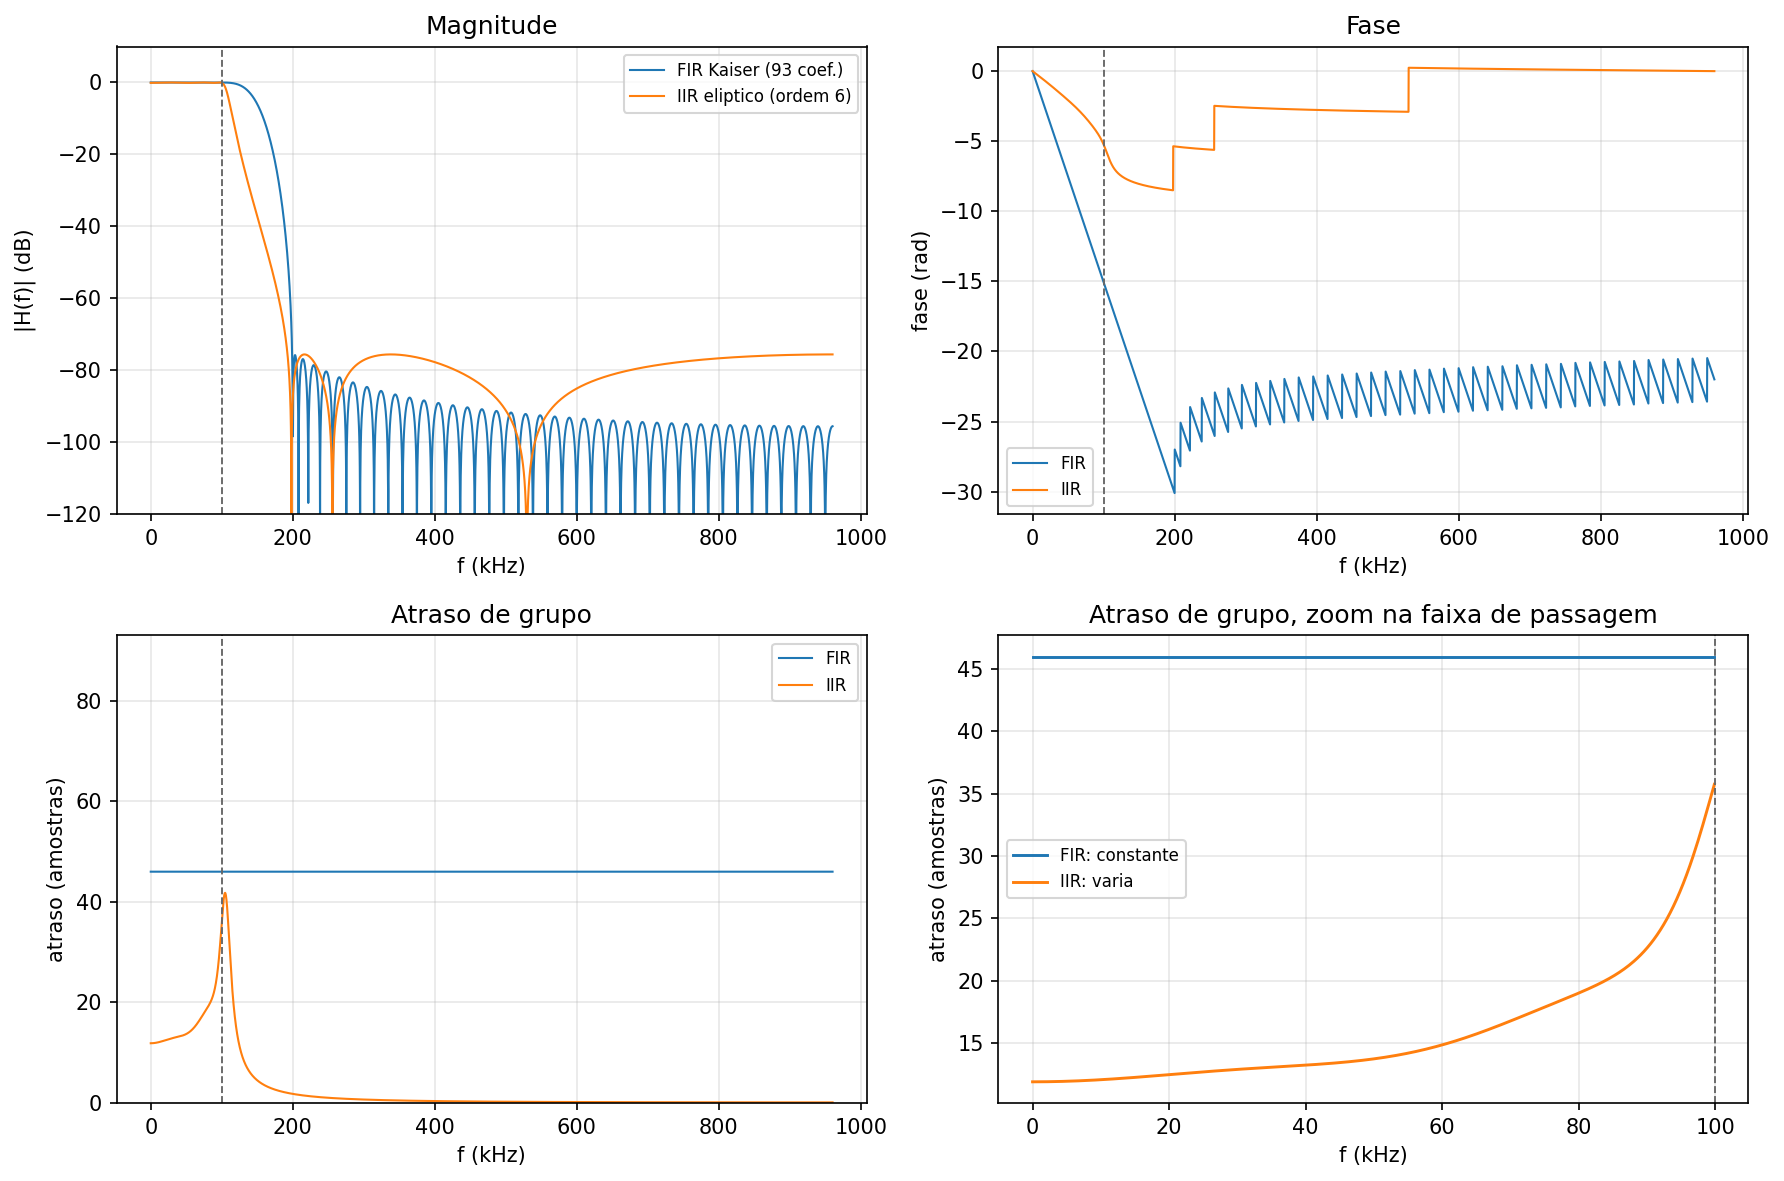
\includegraphics[width=\linewidth]{Imagens/fig06_fir_vs_iir.png}
\label{fig:fir-vs-iir}
\fonte{Autoria própria.}
\end{figure}

O zoom no canto inferior direito é o mais eloquente: uma componente do canal em $100$~kHz sai do filtro IIR quase $24$ amostras depois de uma componente em torno de $0$~Hz. Como o símbolo é formado pela soma de todas essas componentes, ele deixa de chegar inteiro em um instante só — sua energia se espalha, e é isso que borra a constelação. Para corrigir, seria preciso colocar um equalizador passa-tudo em cascata, que devolve a ordem economizada.

O segundo é que o IIR não se decompõe em forma polifásica. A decomposição depende de a saída ser combinação linear apenas das \emph{entradas}. No IIR, cada saída depende das saídas anteriores — inclusive daquelas que o decimador iria descartar. Não existe deixar de calcular três de cada quatro, porque o estado interno do filtro precisa ser atualizado a cada amostra que entra. O IIR fica preso à taxa alta, e o custo por amostra de saída volta a ser multiplicado por $4$: as três seções de segunda ordem custam cerca de $15$ multiplicações por amostra de entrada, o que dá $60$ por amostra de saída. Comparando com as $96$ do FIR polifásico, a economia é de apenas $36$ multiplicações — e o preço são os $23{,}86$ amostras de dispersão no atraso de grupo.

A Tabela~\ref{tab:fir-iir} resume a comparação.

\begin{table}[htb]
\centering
\caption{Comparação entre o FIR projetado e um IIR elíptico equivalente.}
\label{tab:fir-iir}
\begin{tabular}{lcc}
\hline
 & \textbf{FIR Kaiser} & \textbf{IIR elíptico} \\
\hline
Ordem / coeficientes & $93$ coeficientes & ordem $6$ \\
Atraso de grupo na passagem & $46$ amostras (constante) & $11{,}90$ a $35{,}75$ amostras \\
Dispersão do atraso & $0$ & $23{,}86$ amostras ($12{,}42$~$\mu$s) \\
Multiplicações por amostra de saída & $96$ (polifásico) & $60$ (taxa alta) \\
Aceita decomposição polifásica & sim & não \\
Estabilidade & garantida & depende dos coeficientes \\
\hline
\end{tabular}
\fonte{Autoria própria.}
\end{table}

Some-se a isso que o FIR é sempre estável e pouco sensível ao arredondamento dos coeficientes, enquanto um IIR realimentado pode instabilizar ou entrar em ciclo limite quando implementado em aritmética de ponto fixo — um risco real em um receptor embarcado.

\chapter{Conclusão}
\label{cap:conclusao}

O projeto exigia duas tarefas simultâneas: separar o canal de interesse dos canais vizinhos e proteger a decimação por 4 contra o dobramento espectral. Como os sinais eram originados de um sistema SDR e baseados em uma constelação I/Q, o filtro FIR passa-baixas projetado pelo método da janela de Kaiser cumpriu ambas as funções com precisão. Com 93 coeficientes e um atraso de grupo constante de 46 amostras, a solução atendeu a todos os três critérios de aprovação com bastante folga.

Uma situação observada ao responder os questionários foi que a atenuação de $60 dB$ presente na tabela de dados não era suficiente. O critério de aprovação exige que o interferente de $450 kHz$ fique $60 dB$ abaixo do canal útil, mas ele entra no sistema $15,56 dB$ acima dele. Somando essa diferença de entrada ao nível de rejeição exigido, a atenuação real necessária no filtro passa a ser de $75,56 dB$. Desta forma, um filtro projetado com exatamente $60 dB$ seria reprovado nesse requisito.

Na prática, a escolha pelo filtro FIR se mostra totalmente acertada quando analisada em detalhes: embora um filtro IIR elíptico de ordem 6 conseguisse resolver a seletividade com bem menos coeficientes, ele causaria uma variação de 24 amostras no atraso de grupo dentro do canal, borrando a constelação I/Q que o bloco seguinte precisa ler, enquanto o FIR simétrico garante fase linear por construção, mantendo um atraso rigorosamente constante em 46 amostras. Além disso, a arquitetura polifásica demonstra que o alto custo computacional do FIR é facilmente superado, pois ao dividir a filtragem em quatro subfiltros que já operam na taxa reduzida, o número de multiplicações por amostra de saída cai de 372 para 96 sem qualquer aproximação — apresentando uma diferença irrisória de apenas $1{,}5 \times 10^{-15}$ por erro de arredondamento —, o que equipara o custo do FIR polifásico ao de um IIR equivalente, com a grande vantagem de não distorcer a fase e de ser incondicionalmente estável.

Por fim, a comparação dos espectros antes e depois da decimação deixou visível o fenômeno que motivou todo o projeto. Sem filtro, o interferente de $450$~kHz reaparece em $-30$~kHz com $15{,}6$~dB acima do canal útil. Com o filtro aplicado antes do decimador, ele desaparece. A ordem das operações, filtrar primeiro, decimar depois é o que torna a redução de taxa uma operação segura. Foi muito interessante esse projeto pois me ajudou a entender melhor como funciona o Processamento de Sinais, e foi um desafio finaliza-lo e compreender e integrar todo o sistema deste o contexto apresentado, no final foi uma ótima experiência de aprendizado.




% ----------------------------------------------------------
% ELEMENTOS PÓS-TEXTUAIS
% ----------------------------------------------------------
\postextual

% ----------------------------------------------------------
% Referências bibliográficas
% ----------------------------------------------------------
 
\bibliography{referencias}
\nocite{google_gemini_2026} 
\nocite{oppenheim_sinais_2010}
\nocite{marcos_pibiti_2024}
\nocite{anotacoes_aula}
\nocite{anthropic_claude_2026}

\end{document}
